\documentclass[11pt,a4paper]{article}
\usepackage[T1]{fontenc}
\usepackage[margin=2.3cm]{geometry}
\usepackage{amsmath,amssymb}
\usepackage{graphicx}
\usepackage[dvipsnames]{xcolor}
\usepackage{enumitem}
\usepackage[colorlinks=true,linkcolor=blue,urlcolor=blue]{hyperref}
\setlength{\parskip}{0.6em}
\setlength{\parindent}{0pt}
\begin{document}

\begin{center}{\LARGE\bfseries openmotion}\\[0.4em]{\large Read position, velocity and acceleration graphs like a physicist, in three sessions.}\\[0.2em]\small PAN IIT OSS explainer \textbullet{} secondary school to diploma / undergraduate (levels 3-5)\end{center}

\section*{Why this exists}
Every moving body leaves a trail of positions in time. This explainer shows how that one record contains the velocity and the acceleration too, as slopes of graphs, and how to read them even when the data are noisy.

\section*{The end goal}
Read position, velocity and acceleration graphs of a moving body. The end goal is to read position, velocity and acceleration graphs of a moving body: to know what slope and area mean, to use the equations of motion, and to recover speed and acceleration from real measurements. The same ideas run through sports analysis, vehicle testing and every sensor that measures motion.

\section*{How the three sessions build up}
\begin{enumerate}[nosep]
\item \textbf{Session 1: One motion, three graphs: slope and area} (Level 1, conceptual interactive model, 60 min).
\item \textbf{Session 2: Equations of motion, piecewise trips and stopping distance} (Level 2, mathematical engineering model, 75 min).
\item \textbf{Session 3: Differentiating and integrating noisy data} (Level 3, simulation and validation, 90 min).
\end{enumerate}

\section{Session 1: One motion, three graphs: slope and area}

\subsection*{A. Real-world problem}
A car pulls away from a junction. A speed camera records where it is, and you want to know how fast it was going and whether it was speeding up or slowing down. You cannot see speed in a list of positions, but you can see it in a graph: a steep position graph means fast. Why? And if someone gives you only the speed graph, can you work out how far the car went?

\subsection*{B. Concept and theory}
Position x is where the body is along a line (metres). Velocity v is how fast x changes, including direction (metres per second): it is the slope of the x-t graph. Acceleration a is how fast v changes (metres per second squared): it is the slope of the v-t graph. In the other direction, the area between the v-t graph and the time axis is the displacement, and the area under the a-t graph is the change of velocity. Area below the axis counts as negative (motion backwards). For a constant acceleration the three graphs are a parabola, a straight line and a flat line.

\begin{itemize}[nosep]
\item t: time (s)
\item x0: starting position (0 in this session) (m)
\item x: position at time t (m)
\item v0: velocity at t = 0 (m/s)
\item v: velocity at time t (m/s)
\item a: acceleration (constant) (m/s\textasciicircum{}2)
\end{itemize}

\begin{equation*}
a(t)=a,\qquad v(t)=v_0+a\,t,\qquad x(t)=x_0+v_0\,t+\tfrac12 a\,t^2
\end{equation*}

\begin{equation*}
v=\frac{dx}{dt},\qquad a=\frac{dv}{dt}
\end{equation*}

\begin{equation*}
\Delta x=\int_0^t v\,dt',\qquad \Delta v=\int_0^t a\,dt'
\end{equation*}

\begin{center}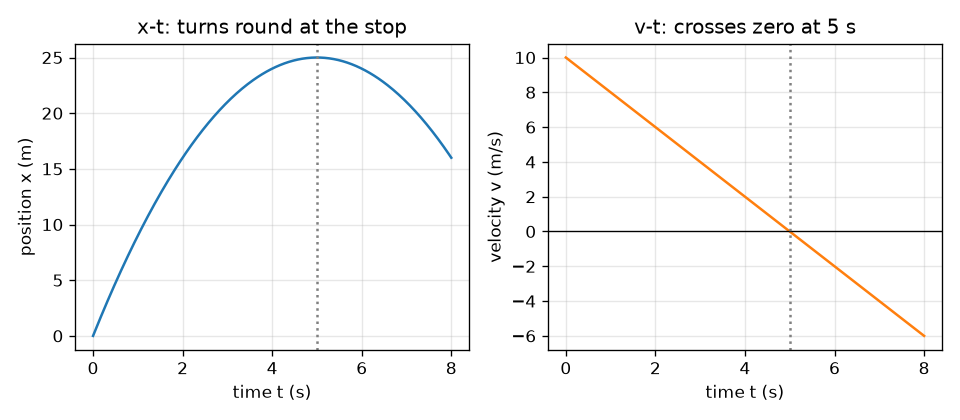
\includegraphics[width=0.85\linewidth]{figures/s01_braking.png}\\\small Braking from 10 m/s at -2 m/s\textasciicircum{}2: the car stops at 5 s and 25 m, and would then reverse.\end{center}

\subsection*{E. Worked example}
A car starts at x = 0 with v0 = 4 m/s and accelerates at 2 m/s\textasciicircum{}2. Find its velocity and position after 5 s, then check the answers with the slope and the area.
\begin{enumerate}[nosep]
\item Velocity: v = v0 + a t = 4 + 2 * 5 = 14 m/s.
\item Position: x = v0 t + (1/2) a t\textasciicircum{}2 = 4 * 5 + 0.5 * 2 * 25 = 20 + 25 = 45 m.
\item Slope check: the slope of the x-t curve at 5 s should be the velocity. A step of 0.001 s either side gives (x(5.001) - x(4.999)) / 0.002 = 14 m/s.
\item Area check: the v-t graph from 0 to 5 s is a trapezoid with parallel sides 4 and 14 m/s and width 5 s: area = (4 + 14) / 2 * 5 = 45 m. The two methods agree.
\end{enumerate}
\textbf{Answer.} v = 14 m/s and x = 45 m after 5 s; the slope of x-t is 14 m/s and the area under v-t is 45 m.

\subsection*{F. Questions}
\begin{enumerate}[nosep]
\item \textbf{Conceptual.} What does the slope of a position-time graph represent? What does a negative slope mean, and what does a flat part mean?
\item \textbf{Numerical.} A car has v0 = 3 m/s and a = 2.5 m/s\textasciicircum{}2. Find its velocity and the distance it has moved after 4 s. Check the units and that the answer is sensible.
\item \textbf{Graph and simulation interpretation.} A v-t graph is a straight line from (0 s, 12 m/s) down to (6 s, 0 m/s). In which direction is the acceleration, what is its value, and how far did the body move?
\item \textbf{Design and optimisation challenge.} Design: a car travelling at 10 m/s must stop within 30 m. What constant deceleration is needed at least, and how long does the stop take? State your assumptions.
\end{enumerate}

\section{Session 2: Equations of motion, piecewise trips and stopping distance}

\subsection*{A. Real-world problem}
A driver sees a hurdle 40 m ahead while the car is doing 20 m/s (72 km/h). The driver needs about a second to react, and the brakes then need distance to work. Does the car stop in time? If not, how fast would it be going when it hits, and what is the fastest speed that would still be safe? This lesson is a simplified model for learning, with constant braking on a dry flat road; real stopping distances depend on tyres, road, load and driver, and the lesson must never be used to decide how to drive.

\subsection*{B. Concept and theory}
For a constant acceleration a, three equations connect v0, v, a, t and the displacement dx. Eliminating t gives v\textasciicircum{}2 = v0\textasciicircum{}2 + 2 a dx, which links speed and distance directly. A stop from speed v at deceleration a (a positive number) takes dx = v\textasciicircum{}2 / (2 a): doubling the speed quadruples the braking distance. During the reaction time t\_r the car keeps its speed and covers v t\_r. A trip is solved piece by piece: the final velocity and position of one piece are the start of the next, and the total displacement is the total area under the v-t graph.

\begin{itemize}[nosep]
\item v0, v: starting and final velocity (m/s)
\item a: acceleration (deceleration in the braking formulas, as a positive number) (m/s\textasciicircum{}2)
\item dx: displacement (m)
\item t\_r: driver reaction time (s)
\item D: distance to the hurdle (m)
\item v\_c: cruise speed of a trip (m/s)
\end{itemize}

\begin{equation*}
v=v_0+a\,t,\qquad \Delta x=v_0 t+\tfrac12 a t^2,\qquad v^2=v_0^2+2a\,\Delta x
\end{equation*}

\begin{equation*}
d_{stop}=v\,t_r+\frac{v^2}{2a}
\end{equation*}

\begin{equation*}
v_{max}=a\left(-t_r+\sqrt{t_r^2+\frac{2D}{a}}\right)
\end{equation*}

\begin{center}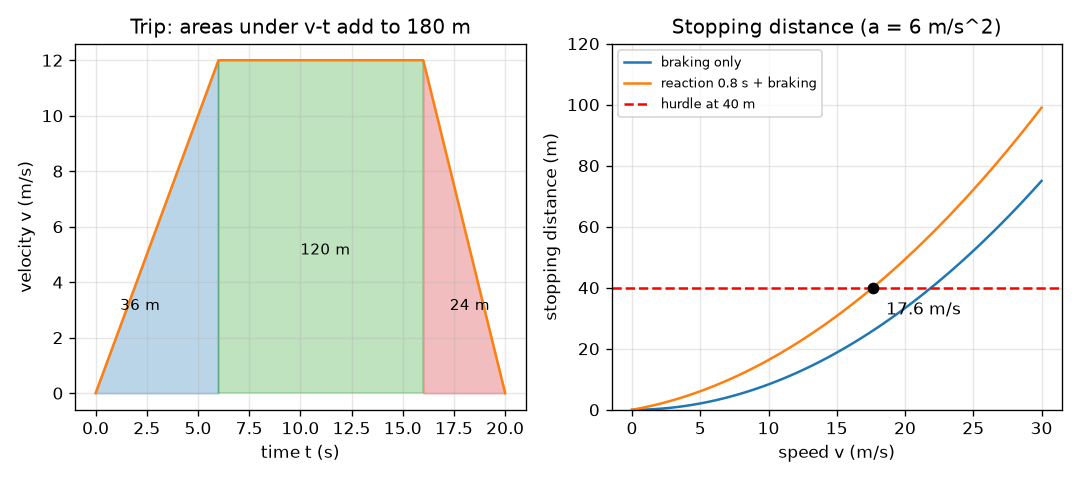
\includegraphics[width=0.85\linewidth]{figures/s02_trip_and_stopping.png}\\\small Left: the areas under the v-t graph of a trip add up to 180 m. Right: stopping distance against speed, and the largest safe speed for a 40 m hurdle.\end{center}

\subsection*{E. Worked example}
A trip: speed up from rest at 2 m/s\textasciicircum{}2 to 12 m/s, cruise for 10 s, then brake to rest at 3 m/s\textasciicircum{}2. Find the time and distance of each piece, the total distance and the average speed.
\begin{enumerate}[nosep]
\item Speeding up: t1 = v\_c / a = 12 / 2 = 6 s; distance = 0.5 * 12 * 6 = 36 m (area of a triangle).
\item Cruising: distance = 12 * 10 = 120 m (area of a rectangle), taking 10 s.
\item Braking: t3 = 12 / 3 = 4 s; distance = 0.5 * 12 * 4 = 24 m.
\item Total distance = 36 + 120 + 24 = 180 m in 6 + 10 + 4 = 20 s.
\item Average speed = 180 / 20 = 9 m/s, lower than the cruise speed because of the slow ends.
\item Intervals of acceleration from the graph: positive (+2 m/s\textasciicircum{}2) from 0 to 6 s, zero from 6 to 16 s, negative (-3 m/s\textasciicircum{}2) from 16 to 20 s.
\end{enumerate}
\textbf{Answer.} 180 m in 20 s, average speed 9 m/s; accelerating 0 to 6 s, cruising 6 to 16 s, braking 16 to 20 s.

\subsection*{F. Questions}
\begin{enumerate}[nosep]
\item \textbf{Conceptual.} Why does the braking distance grow with the square of the speed, while the reaction distance grows only in proportion to it? What happens to the braking distance if the speed doubles?
\item \textbf{Numerical.} A car at 15 m/s brakes with a deceleration of 5 m/s\textasciicircum{}2. Find the braking time and distance. If the driver also takes 1.0 s to react, what is the total stopping distance?
\item \textbf{Graph and simulation interpretation.} Using the stopping-distance graph (reaction time 0.8 s, a = 6 m/s\textasciicircum{}2), at what speed does the car just stop at the 40 m hurdle? At 20 m/s, which is larger, the reaction distance or the braking distance?
\item \textbf{Design and optimisation challenge.} Design: the hurdle is 40 m away and the braking deceleration cannot exceed 6 m/s\textasciicircum{}2. Find the largest safe speed for a reaction time of 0.8 s, and for a quicker driver with 0.5 s. What does the comparison tell you about the design?
\end{enumerate}

\section{Session 3: Differentiating and integrating noisy data}

\subsection*{A. Real-world problem}
A phone camera or a GPS gives you positions at fixed time steps, each a little wrong. You want velocity and acceleration, which are slopes of slopes. A tiny error of 2 cm in position becomes an error of 0.3 m/s in velocity and almost 20 m/s\textasciicircum{}2 in acceleration, more than the real acceleration. How can we tame this, and how do we know the answer is right? We test every method on a motion whose exact answer we know. This is a simplified model of measurement noise and is for learning.

\subsection*{B. Concept and theory}
Sampled positions x\_i are taken every dt seconds. The centred difference (x[i+1] - x[i-1]) / (2 dt) estimates the velocity and the second difference (x[i+1] - 2 x[i] + x[i-1]) / dt\textasciicircum{}2 the acceleration. Two errors appear. Truncation error comes from the formula itself and shrinks like dt\textasciicircum{}2. Noise error comes from random errors in x: if each x has standard deviation sigma, the velocity error is about sigma / (sqrt(2) dt) and the acceleration error about sqrt(6) sigma / dt\textasciicircum{}2, so smaller dt makes noise worse. Fitting a cubic polynomial to the 2h + 1 samples around each point and using the slope or curvature of the fit averages many samples and cuts the noise, at the price of blurring real changes if the window is too wide. Integration goes the other way: adding up many samples averages the noise out.

\begin{itemize}[nosep]
\item dt: time between samples (s)
\item sigma: standard deviation of the position noise (m)
\item x\_i: measured position of sample i (m)
\item h: half window: the fit uses 2h + 1 samples (samples)
\item v\_est, a\_est: estimated velocity and acceleration (m/s, m/s\textasciicircum{}2)
\item RMS error: square root of the mean squared difference from the exact value (same as the quantity)
\end{itemize}

\begin{equation*}
v_i\approx\frac{x_{i+1}-x_{i-1}}{2\,\Delta t},\qquad a_i\approx\frac{x_{i+1}-2x_i+x_{i-1}}{\Delta t^2}
\end{equation*}

\begin{equation*}
\sigma_v\approx\frac{\sigma}{\sqrt2\,\Delta t},\qquad \sigma_a\approx\frac{\sqrt6\,\sigma}{\Delta t^2}
\end{equation*}

\begin{equation*}
\left|v_i-v(t_i)\right|\le\frac{\Delta t^2}{6}\max|x'''|\quad\text{(no noise)}
\end{equation*}

\begin{center}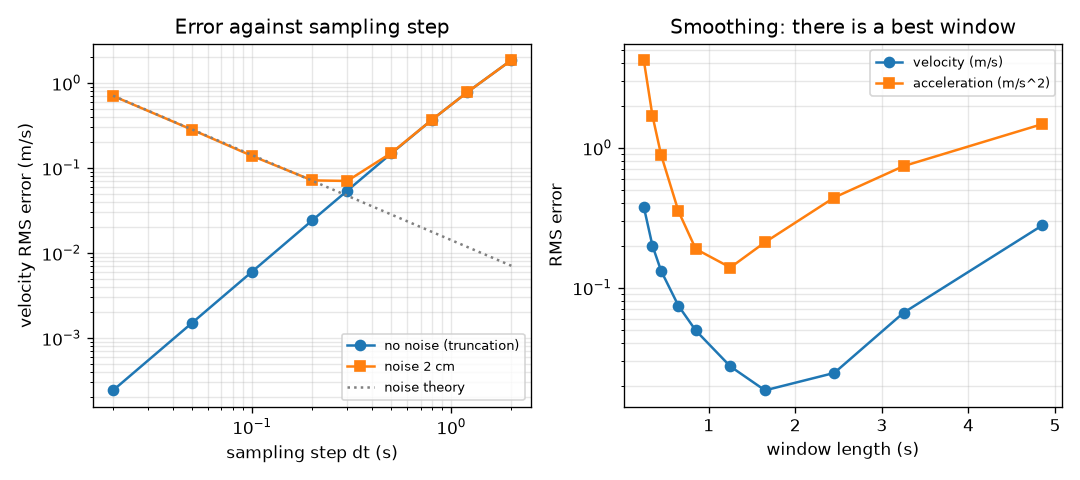
\includegraphics[width=0.85\linewidth]{figures/s03_error_sensitivity.png}\\\small Velocity error against the sampling step (left) and against the smoothing window (right).\end{center}

\subsection*{E. Worked example}
For dt = 0.05 s and sigma = 0.02 m, predict the velocity and acceleration errors of plain finite differences, then measure them on simulated data, then smooth with a 17-point cubic fit (h = 8).
\begin{enumerate}[nosep]
\item Predicted velocity error: sigma / (sqrt(2) dt) = 0.02 / (1.414 * 0.05) = 0.283 m/s.
\item Predicted acceleration error: sqrt(6) sigma / dt\textasciicircum{}2 = 2.449 * 0.02 / 0.0025 = 19.6 m/s\textasciicircum{}2, which is 4.5 times the real wiggle of 4.32 m/s\textasciicircum{}2.
\item Measured on 401 simulated samples (seed 1): velocity RMS error 0.274 m/s and acceleration RMS error 19.24 m/s\textasciicircum{}2, within 10 percent of the predictions.
\item Truncation check without noise: the error stays below dt\textasciicircum{}2 / 6 * 3 * 1.2\textasciicircum{}3 = 0.00216 m/s (measured largest error 0.00216 m/s, just under the bound).
\item Smoothing with h = 8 (window 0.85 s): velocity error 0.040 m/s and acceleration error 0.16 m/s\textasciicircum{}2, about 7 and 120 times smaller.
\end{enumerate}
\textbf{Answer.} Plain differences: 0.28 m/s and 19.6 m/s\textasciicircum{}2 predicted, 0.27 m/s and 19.2 m/s\textasciicircum{}2 measured. A 17-point cubic fit cuts them to 0.04 m/s and 0.16 m/s\textasciicircum{}2.

\subsection*{F. Questions}
\begin{enumerate}[nosep]
\item \textbf{Conceptual.} Why is differentiating noisy data much worse than integrating it? Explain with one sentence about what each operation does to random errors.
\item \textbf{Numerical.} For sigma = 0.02 m, predict the noise errors of the velocity and the acceleration if the sampling step is halved from 0.05 s to 0.025 s. By what factors do they change?
\item \textbf{Graph and simulation interpretation.} On the error-against-step graph (velocity, central difference), why does the noisy curve have a minimum near dt = 0.3 s? What happens at dt = 2 s even without noise?
\item \textbf{Design and optimisation challenge.} Design: with sigma = 0.02 m and dt = 0.05 s, choose a window length for the local cubic fit so that the acceleration error is below 0.5 m/s\textasciicircum{}2. Which windows work, and what is the trade-off?
\end{enumerate}

\section{Real-world mini-project}
\textbf{Analyse a motion recorded by a phone.} Film a trolley, a toy car or a person walking past a ruler with your phone (30 frames per second is typical), and read its position from the frames, or log positions with any phone app you like. Start with the synthetic example \texttt{phone\_dataset()} in Session 3: a trolley that speeds up, cruises and brakes, filmed at 30 frames per second with 2 cm position error. Estimate its velocity and acceleration with \texttt{smooth\_derivative}, choose the window yourself, and then repeat with your own recording.

\section{The path ahead}
\begin{enumerate}[nosep]
\item \textbf{Session 4: Fit the pieces, not the points.} A change-point fit of the three pieces of a noisy trip.
\item \textbf{Session 5: Let the data choose the window.} A function that picks the smoothing window without knowing the true motion.
\item \textbf{Session 6: Error bars on velocity.} A 95 percent interval drawn around the recovered velocity.
\item \textbf{Session 7: Your own phone recording.} A recording of a rolling trolley analysed end to end.
\item \textbf{Session 8: A tossed ball in two dimensions.} The analysis of a ball toss filmed side-on.
\end{enumerate}

\section{Answers and hints}

\subsection*{Session 1}
\begin{enumerate}[nosep]
\item \textbf{Conceptual.} Hint: Slope is rise over run. What is the rise and what is the run? Solution: The rise is a change of position and the run is a change of time, so the slope is change of position per unit time: the velocity. A negative slope means the position is decreasing, so the body moves backwards (opposite to the positive direction). A flat part has zero slope: the body is at rest.
\item \textbf{Numerical.} Hint: Use v = v0 + a t and x = v0 t + (1/2) a t\textasciicircum{}2. Solution: v = 3 + 2.5 * 4 = 13 m/s. x = 3 * 4 + 0.5 * 2.5 * 16 = 12 + 20 = 32 m. Units: (m/s)(s) = m and (m/s\textasciicircum{}2)(s\textasciicircum{}2) = m. Sanity check: the average velocity is (3 + 13) / 2 = 8 m/s, and 8 m/s * 4 s = 32 m. The numbers agree.
\item \textbf{Graph and simulation interpretation.} Hint: The slope gives the acceleration; the area of the triangle gives the distance. Solution: The line goes down, so the acceleration is negative (the body is slowing down while moving forward): a = (0 - 12) / 6 = -2 m/s\textasciicircum{}2. The area is a triangle: 0.5 * 6 s * 12 m/s = 36 m. The body moved 36 m forward and stopped.
\item \textbf{Design and optimisation challenge.} Hint: The v-t graph is a triangle with area equal to the stopping distance. Solution: The area of the triangle is 0.5 * 10 * T = 30, so T = 6 s and the deceleration is 10 / 6 = 1.67 m/s\textasciicircum{}2 (a bit more would be safer). Check: the 'no time' formula gives v\textasciicircum{}2 / (2 d) = 100 / 60 = 1.67 m/s\textasciicircum{}2. Assumptions: constant deceleration from the first instant, a straight road, no reaction time (Session 2 adds it).
\end{enumerate}

\subsection*{Session 2}
\begin{enumerate}[nosep]
\item \textbf{Conceptual.} Hint: Compare v t\_r with v\textasciicircum{}2 / (2 a). Solution: During the reaction time the car moves at constant speed, so the distance is speed times time: proportional to v. Braking removes speed at a fixed rate, so a faster car takes longer to stop and also covers more distance every second: the distance is v\textasciicircum{}2 / (2 a). Doubling the speed doubles the reaction distance but multiplies the braking distance by 4.
\item \textbf{Numerical.} Hint: t = v / a, and dx = v\textasciicircum{}2 / (2 a). Solution: Braking time = 15 / 5 = 3 s. Braking distance = 15\textasciicircum{}2 / (2 * 5) = 225 / 10 = 22.5 m. Reaction distance = 15 * 1.0 = 15 m. Total = 37.5 m. Sanity check: the average speed while braking is 7.5 m/s, and 7.5 * 3 = 22.5 m.
\item \textbf{Graph and simulation interpretation.} Hint: Find where the upper curve meets the red line; then compare 20 * 0.8 with 400 / 12. Solution: The curve meets the 40 m line at about 17.6 m/s (63.5 km/h). At 20 m/s the reaction distance is 20 * 0.8 = 16 m and the braking distance is 400 / 12 = 33.3 m, so braking is the larger part, and the total is 49.3 m, over the hurdle by 9.3 m.
\item \textbf{Design and optimisation challenge.} Hint: Solve v t\_r + v\textasciicircum{}2 / (2 a) = D for v: v = a (-t\_r + sqrt(t\_r\textasciicircum{}2 + 2 D / a)). Solution: For t\_r = 0.8 s: v = 6 * (-0.8 + sqrt(0.64 + 13.33)) = 6 * (-0.8 + 3.738) = 17.63 m/s. For t\_r = 0.5 s: v = 6 * (-0.5 + sqrt(0.25 + 13.33)) = 6 * (-0.5 + 3.685) = 19.11 m/s. Trade-off: 0.3 s less reaction time buys about 1.5 m/s of speed, but no reaction time can make 20 m/s safe with 6 m/s\textasciicircum{}2 over only 40 m (braking alone needs 33.3 m, leaving just 6.7 m for reaction = 0.33 s). Design options: a lower speed limit, an earlier warning sign, or better brakes. Assumption: constant braking on a dry road.
\end{enumerate}

\subsection*{Session 3}
\begin{enumerate}[nosep]
\item \textbf{Conceptual.} Hint: Think of a slope between two points that are close together, and of a sum of many points. Solution: A slope divides the difference of two noisy numbers by a small time step, so the error is magnified by roughly 1/dt, and taking a slope again magnifies it by another 1/dt. Integrating adds many samples times dt, and random errors of both signs partly cancel, so the total error grows slowly. In the lesson, integrating a velocity with 0.2 m/s noise over 20 s left a position error of only 0.12 m.
\item \textbf{Numerical.} Hint: Use sigma / (sqrt(2) dt) and sqrt(6) sigma / dt\textasciicircum{}2. Solution: Velocity: 0.02 / (1.414 * 0.025) = 0.566 m/s, twice as large as 0.283. Acceleration: 2.449 * 0.02 / 0.000625 = 78.4 m/s\textasciicircum{}2, four times as large as 19.6. Halving dt makes the noise worse by a factor 2 for v and 4 for a. Sanity check: both errors scale with a negative power of dt.
\item \textbf{Graph and simulation interpretation.} Hint: Two error sources compete. Which one wins at small dt and which at large dt? Solution: Noise error falls like 1/dt and truncation error rises like dt\textasciicircum{}2; they are equal where 0.02 / (1.414 dt) = 0.61 dt\textasciicircum{}2, i.e. dt = 0.28 s, so the sum is smallest near 0.3 s (0.070 m/s measured). At dt = 2 s the sampling is nearly as slow as the 5.2 s wiggle of the motion, so a centred difference misses it: the velocity error is 1.85 m/s even with no noise at all. This is the sampling limit.
\item \textbf{Design and optimisation challenge.} Hint: Use the table printed by the lesson (error against half window). Solution: From the lesson table (average of 10 noise seeds), windows from about 0.65 s (error 0.35 m/s\textasciicircum{}2) to 2.45 s (0.44 m/s\textasciicircum{}2) are under 0.5; the best is near 1.25 s (0.14 m/s\textasciicircum{}2). Shorter windows keep the noise (0.25 s gives 4.2 m/s\textasciicircum{}2), longer ones blur the real 5.2 s wiggle (4.85 s gives 1.5 m/s\textasciicircum{}2). A window of about 1.25 s, the quarter of the wiggle period, is a good choice. Trade-off: a wide window is calm but would blur the sharp corners of a trip. Assumption: smooth motion and independent noise.
\end{enumerate}

\section{How to join}
Read \texttt{CONTRIBUTING.md} in the repository, then pick an issue labelled \texttt{good first issue}. Repository: \url{https://github.com/KrunalPanchal1995/openmotion}

\end{document}
